\documentclass[openany, notitlepage, justified]{tufte-book}
\usepackage{amsmath, amssymb, amsthm, bm}
\usepackage{graphicx, epsdice, xcolor, listings}

\geometry{                                                                      
    height=11.0in,                                                              
    width=8.5in,                                                                
    left=1in, % left margin                                                     
    textwidth=5.2in, % main text block                                          
    marginparsep=0.2in, % gutter between main text block and margin notes       
    marginparwidth=1.6in % width of margin notes                                
}    

\usepackage{etoolbox}
\makeatletter
\patchcmd{\chapter}{\if@openright\cleardoublepage\else\clearpage\fi}{}{}{}
\makeatother

\newcommand{\EE}{\mathbb{E}}
\newcommand{\PP}{\mathbb{P}}
\newcommand{\RR}{\mathbb{R}}
%
\newcommand{\Dd}{\mathcal{D}}
\newcommand{\Ee}{\mathcal{E}}
\newcommand{\Gg}{\mathcal{G}}
\newcommand{\Hh}{\mathcal{H}}
\newcommand{\Ii}{\mathcal{I}}
\newcommand{\Ll}{\mathcal{L}}
\newcommand{\Ss}{\mathcal{S}}
\newcommand{\Xx}{\mathcal{X}}
\newcommand{\Yy}{\mathcal{Y}}

\newcommand{\sdia}[1]{%
    \begingroup%
    \setbox0=\hbox{\includegraphics[height=\baselineskip]{#1}}%
    \parbox{\wd0}{\box0}\endgroup%
}

\newcommand{\Ein}{\Ee_{\text{in},\Ss}}
\newcommand{\Einb}{\Ee_{\text{in},\tilde\Ss}}
\newcommand{\Einc}{\Ee_{\text{in},\Ss\cup\tilde\Ss}}
\newcommand{\Eout}{\Ee_{\text{out}}}

\begin{document}

    \begin{adjustwidth}{0in}{-1.3in}
    \begin{center}
        \Huge 
        Generalization in Machine Learning \\
        \large         
        Sam, Arthur, and Joe ~~~~~~~~~~ 2020 Summer
    \end{center}
    \end{adjustwidth}

    \chapter{The Cake Problem}
        \section{A tempting pattern}
            We'll start out with a fun puzzle that's not directly related to
            machine learning but whose math will later help us.
            %
            Imagine $n$ people are seated around a large disk-shaped cake.
            Each pair of people will use a two-person handsaw to cut the cake.
            For example, the picture below shows a group of $4$ people; there
            are $6$ pairs of people, so the group makes $6$ cuts total.  With
            $4$ people, the cake ends up in $8$ pieces.  We
            wonder: how many pieces arise when more people sit
            around the cake?
            %
            \begin{marginfigure}
                \centering
                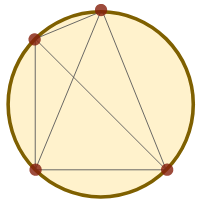
\includegraphics[height=3cm]{cake-4}
                \caption{\emph{
                    With $n=4$ people, we make ${n\choose 2}=6$ cuts.  We get
                    $8$ pieces in total ($4$ outside and $4$ inside).  
                }}
            \end{marginfigure}

            Here are some drawings for possibilities ranging from $n=1$ people
            to $n=6$ people.  Try counting the pieces and guessing a pattern!
            Can you find a formula for how many pieces arise when there are $n$
            people?
            \begin{figure}[h!]
                \centering
                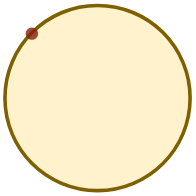
\includegraphics[height=3cm]{cake-1}
                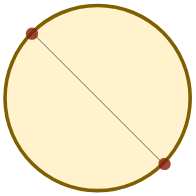
\includegraphics[height=3cm]{cake-2}
                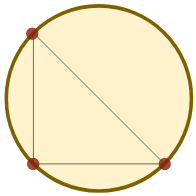
\includegraphics[height=3cm]{cake-3} \\
                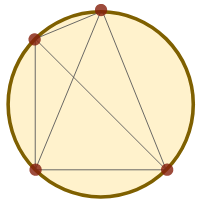
\includegraphics[height=3cm]{cake-4}
                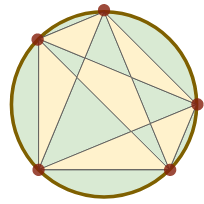
\includegraphics[height=3cm]{cake-5-col}
                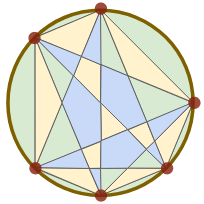
\includegraphics[height=3cm]{cake-6-col}
                \caption{\emph{
                    Here, we color some of the cake pieces just to make them
                    easier to see and to count.
                    %
                    The $n=1$ case doesn't have any cuts.
                    %
                    The $n=5$ case has $5$ outside green pieces, $5$ inside
                    green pieces, $5$ yellow triangles --- so far this is three
                    fives, which makes fifteen --- and what's left is $1$
                    yellow center piece.
                    %
                    The $n=6$ case has $6$ outside green pieces, $6$ inside
                    green pieces, $6$ outer yellow triangles, $6$ blue
                    triangles --- so far this is four sixes, which makes twenty
                    four --- and what's left are the $7$ central blue and
                    yellow shapes.
                }}
            \end{figure}

            Well, it seems that with $n=1, 2, 3, 4$ people, there are $p(n) =
            1, 2, 4, 8$ pieces.  (Here, $p$ stands for ``pieces'', and we'll
            use this way of writing just to save time).  It seems that $p(n)$
            doubles for each next $n$, meaning that $p$ looks like powers of
            two.  In symbols, our guess is: $p(n) \stackrel{?}{=} 2^{n-1}$.

            Let's check this guess.  Does it continue to $n=5$?  We expect the
            next power of two: $8+8=16$.  And yes: $p(5)$ really is
            $16$!  How about $n=6$?  We expect $16+16=32$.  But --- uh oh! ---
            it seems that there are only $31$ pieces.  The pattern breaks.

        \section{An explanation}
            Let's now figure out $p(n)$ for any $n$; along the way, we'll see
            why the powers-of-two pattern seemed to work until $n=6$.
            %
            There are two steps: we'll relate cake to constellations
            and then relate constellations to counting.

            We'll use \textbf{Euler's formula}, which says
            that if we connect a bunch of dots by edges to enclose
            regions, then the numbers of dots, edges, and regions are related:
            $$
                \text{Regions} - \text{Edges} + \text{Dots} = 1
            $$
            For example, the constellation that we build up in stages below
            has $3$ regions (one pentagon and two triangles), $13$ edges, and
            $11$ dots.  And $3-13+11 = 1$, just like the formula says.
            %
            \begin{figure}[h!]
                \centering
                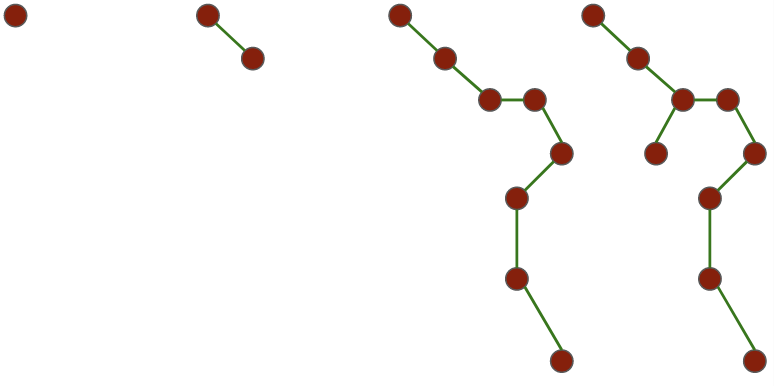
\includegraphics[height=2.7cm]{euler-a}
                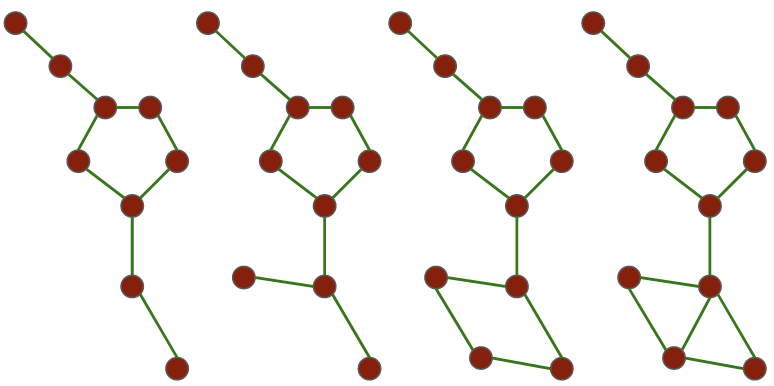
\includegraphics[height=2.7cm]{euler-b}
                \caption{\emph{
                    Steps to build an example constellation (right) starting
                    from a single dot (left).
                    %
                    By the way, this method only helps us build constellations
                    that don't have crossing edges, and each two of whose dots
                    are connected by a path of edges.  Euler's formula only
                    applies to constellations that follow these rules.
                }}
            \end{figure}
            %
            Why is the formula true?  Well, we can build up our constellation
            from a single dot.  The dot follows the formula
            (there are no regions and no edges, and $0-0+1 = 1$).  And
            each step of building keeps the formula true:
            %
            \textbf{either} we connect a new dot to an old dot (so both
            $-\text{Edges}$ and $+\text{Dots}$ change by one, preserving the
            total)
            %
            \textbf{or} we connect two old dots to create a new region (so both
            $\text{Regions}$ and $-\text{Edges}$ change by one, preserving the
            total).  This logic proves Euler's formula. 

            To wrap up, let's think of a cake as a constellation as shown
            below.  In addition to $n$ outer dots, there are ${n \choose 4}$
            inner dots, because from each inner dot emanate $4$ rays pointing
            toward $4$ outer dots.  By similar logic, the number of edges is $n
            + 2{n\choose 2}/2 + 4{n \choose 4}/2$, since there are $n$ outer
            arcs (green), $2{n\choose 2}$ straight-half edges (blue) between
            outer dots, and $4$ half-edges (orange) emanating from each of
            ${n\choose 4}$ inner dots.
            %
            \begin{figure}[h!]
                \centering
                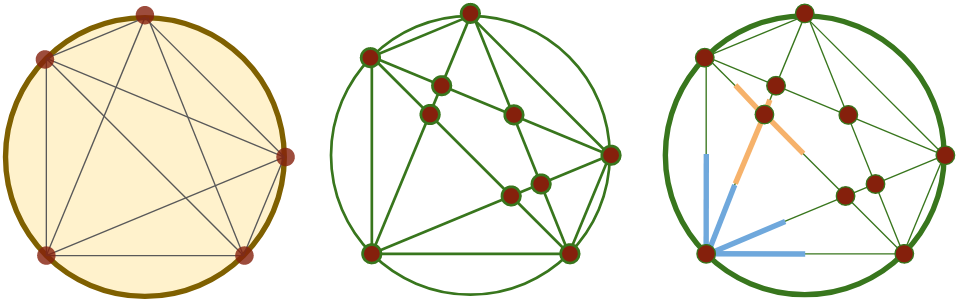
\includegraphics[height=3cm]{count}
                \caption{\emph{
                    We can think of a cake (left)
                    as a constellation (middle) by adding inner dots.
                    We can count the half-edges of the constellation (right) 
                    by binning them into three groups: the outer arcs (green),
                    the straight half-edges between outer dots (blue), and the
                    straight half-edges emanating from inner dots (orange).
                }}
            \end{figure}

            \noindent
            Putting the pieces together, we see
            $
                \text{Regions} = 1 + \text{Edges} - \text{Dots}
                               = 1 + {n\choose 2} + {n\choose 4}
            $.
            We can simplify this by noting that $1={n-1 \choose 0}$ and ${n
            \choose k} = {n-1 \choose k-1} + {n-1 \choose k}$, so
            \begin{align*}
                \text{Regions}
                              = {n-1 \choose 0}
                              + {n-1 \choose 1}
                              + {n-1 \choose 2}
                              + {n-1 \choose 3}
                              + {n-1 \choose 4}
            \end{align*}
            In other words, the number $p(n)$ of pieces for $n$ people equals
            the number of subsets of $n-1$ people with at most $4$ members.
            This explains why we saw powers of two for small $n$: for $n\leq 5$,
            counting small subsets is the same as counting all subsets!
 
    \newpage
    \chapter{What is Learning?}
        \section{Learning to classify}
            Today, we'll analyze machines that learn to classify images into
            two possible buckets such as Cow and Dog.\footnote{
                Our discussion extends to more complicated situations, but
                we'll focus on the simple case.  
            }
            To benefit from math, we need a precise set-up.  What do we mean
            by ``learning to classify''?

            Say $\Xx$ contains all possible images and
            $\Yy=\{\text{Cow},\text{Dog}\}$ is the set of buckets.  We posit a
            probability distribution $\Dd$ over $\Xx \times \Yy$ that says
            which pairs $(x,y)\in \Xx\times \Yy$ are more likely and which are
            less likely.  For instance: we might have $\sdia{cow-a},
            \sdia{cow-d},\cdots \in \Xx$, and $\Dd$ might say that
            %
            $(\sdia{cow-a}, \text{Cow})$ is more likely to occur in nature than 
            $(\sdia{cow-d}, \text{Cow})$, which is more likely to occur than
            $(\sdia{cow-d}, \text{Dog})$, which in turn is more likely than
            $(\sdia{cow-a}, \text{Dog})$.

            A \textbf{classifier} is then a function from images to
            buckets, that is, some $f\in \Yy^{\Xx}$.  By \textbf{learning}, we
            mean acquiring information about $\Dd$ from ``training samples''
            $\Ss \in (\Xx\times\Yy)^N$ drawn independently from $\Dd$.  So
            ``learning to classify'' means mapping $\Ss$s to $f$s.  In
            particular, an \textbf{algorithm} is a function
            $\Ll:(\Xx\times\Yy)^N\to \Yy^{\Xx}$.\footnote{ 
                By the way, we don't have to know $\Dd$ in order to apply our
                theory; we just named it in order to reason about it.
            }

            Instead of considering all possible classifiers, we usually limit
            ourselves to some subset $\Hh \subseteq \Yy^{\Xx}$ of especially
            nice, ``candidate'' classifiers.
            %
            As an example, $\Hh$ might have just three elements:
            \begin{align*}
                \Hh = \{
                    &\text{always say Cow}, \\
                    &\text{say Cow if $x$ is brown on average
                        and otherwise say Dog}, \\
                    &\text{say Cow if
                        $x \in \{\sdia{cow-b}, \sdia{cow-c}, \sdia{cow-e}\}$
                        and otherwise say Dog}
                \}
            \end{align*}
            In practice, $\Hh$ might actually be a much bigger set of neural
            networks.
            %
            \begin{figure}[h!]
                \centering
                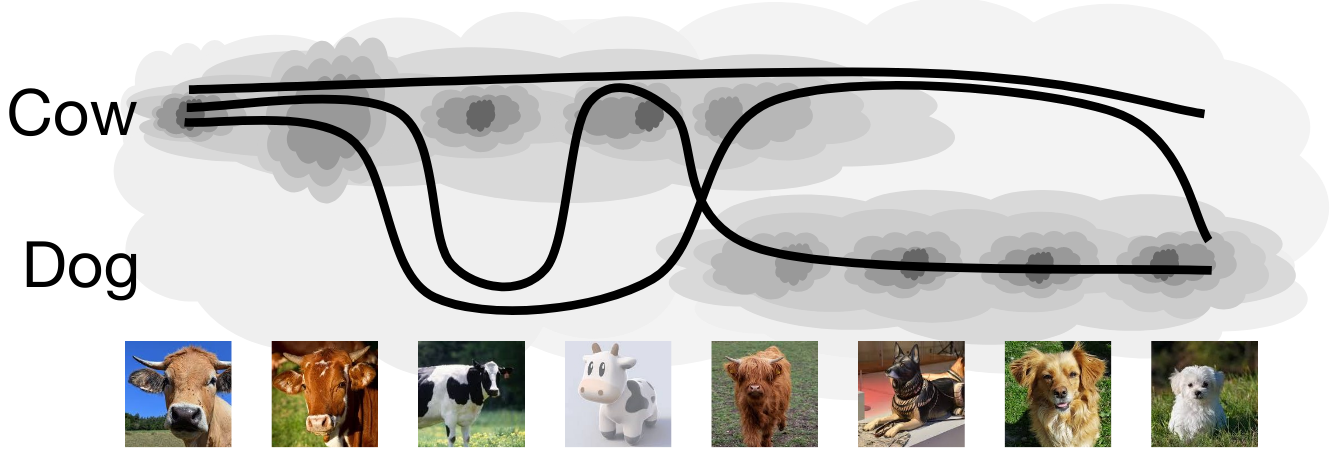
\includegraphics[height=3cm]{hd}
                \caption{\emph{
                    A cartoon of $\Dd$ (clouds) and $\Hh$ (curves) with
                    the $\Xx$ axis horizontal and the $\Yy$ axis vertical. 
                }}
            \end{figure}

        \newpage
        \section{When is an algorithm good?}
            An algorithm $\Ll$ is good when $\Ll(\Ss)$ accurately classifies
            images freshly drawn from $\Dd$.  Notice that this is different
            from merely asking that $\Ll(\Ss)$ accurately classifies the
            elements of $\Ss$!  To notate this difference, we define the
            \textbf{out-error} and \textbf{in-error} (also called the test and
            train errors) of a candidate $f \in \Hh$
            as
            $$
                \Eout(f) = \PP_{(x,y)\sim\Dd} \left[
                               f(x) \neq y
                           \right]
                ~~~~~~~~~~
                \Ein(f) = \PP_{(x,y)\sim\Ss} \left[
                              f(x) \neq y
                          \right]
            $$
            Likewise, the out- and in-errors of a algorithm are
            $
                \Ee_{\cdots}(\Ll) = \Ee_{\cdots}(\Ll(\Ss)) 
            $ where $\Ss\sim\Dd$.

            We hope $\Eout$ is low, but we don't know
            $\Eout$: from $\Ss$, we can directly calculate only
            $\Ein$.  Intuiting that
            $ 
                \Ee_{\text{gap},\Ss} = \Eout - \Ein
            $ 
            tends to be small, we might design $\Ll$ to minimize $\Ein$.
            That is, $\Ll$ computes $\Ein(f)$ for
            each $f\in \Hh$, then (breaking ties arbitrarily) to settle on an
            $f$ with the least $\Ein$.\footnote{
                This $\Ll$ is called \textbf{ERM}; its variants dominate modern
                machine learning.
            }
            
            This $\Ll$ will work when $\Ee_{\text{gap},\Ss}$ is small.
            But is $\Ee_{\text{gap},\Ss}$ actually small?  In particular, if
            $\Ll(\Ss)$ accurately classifies its training samples, will it also
            accurately classify test samples it has never before seen?

            Sometimes, the answer is \textbf{yes}.
                If there is $1$ candidate $f\in \Hh$ and a thousand
                datapoints, then $\Ee_{\cdots}(\Ll) = \Ee_{\cdots}(f)$, and
                $\Ein(f)$ will very probably be very close to
                $\Eout(f)$.  A technical reason for this is that
                $\Ll(\Ss)$ and $\Ss$ are independent, and we may apply the law
                of large numbers.  It's as if we roll a fair die a thousand
                times: we'd expect about a sixth of the rolls to land on
                \epsdice{5}.

            Other times, the answer is \textbf{no}.
                If every possible classifier is a candidate (so $\Hh$ is very
                infinite) and only a few datapoints, then for any training
                sequence $\Ss$, many candidates will perfectly classify the
                training samples.  Say that $\Ll$ breaks ties 
                by settling on
                $$
                    f(x) = \text{say Cow if $(x,\text{Cow}) \in \Ss$;
                            otherwise, say Dog}
                $$
                The problem (assuming each image appears with negligible chance
                and that Cows occur with non-negligible chance) is $f$ will
                misclassify every fresh image of a Cow as a Dog, so it will
                have a huge out-error!  It's as if we do a trillion experiments
                where in each experiment we roll a fair die a thousand times:
                in any one experiment, we'd expect about a sixth of the rolls
                to land on \epsdice{5}, but if we focus on the experiment that
                has the most \epsdice{5}s (which is like focusing on the
                candidates that do the best on the training data), we are
                likely to focus on an outlier that has disproportionately many
                \epsdice{5}s!

            These two examples illustrate that $\Ll$'s training performance
            generalizes to test time when $\Ll$ uses lots of datapoints to
            select from only a small set of candidates.  
            %
            How do these forces balance, for example if there are a lot of
            candidates and also a lot of datapoints?  Let's find out.

            \newpage
    \chapter{Is Learning Possible?}
        \section{A single candidate}
            Let's analyze the case $|\Hh|=1$ more closely.  We write $p$ as
            shorthand for $\Eout(f)$; then $\Ein$
            counts the fraction of heads that appear in $N$ independent flips
            of a coin that has chance $p$ of landing heads.  Intuitively
            $\Ein$ will usually be close to $p$ when $N$ is big.
            Let's make ``usually'', ``close to'', and ``big''  precise.

            \begin{figure}[h!]
                \centering
                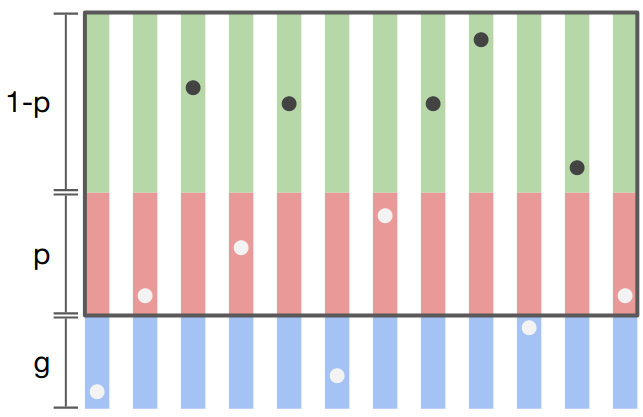
\includegraphics[height=4cm]{chernoff}
                \caption{\emph{
                    We randomly select points on $N$ vertical sticks.  Each
                    stick has three parts: \textbf{green} with length $1-p$,
                    \textbf{red} with length $p$, and \textbf{blue} with length
                    $g$.  We call non-blue points \textbf{boxed} and non-green
                    points \textbf{hollow}.
                }}
            \end{figure}

            We'll switch viewpoints: flipping a coin is like choosing a boxed
            point on a stick where green means tails and red means heads.
            %
            We'll show that probably at most $M_0 = (p+g)N$ heads
            appear.  That is, we want to show --- given that all points are
            boxed --- that probably at most $M_0$ points are red. 
            %
            For any $M\geq M_0$:
            \begin{align*}
                    & ~ \PP[\text{$M$ are red $\mid$ all are boxed}] \\
                  = & ~ \PP[\text{$M$ are red and all are boxed}] ~/~ 
                        \PP[\text{all are boxed}]  \\
                  = & ~ \PP[\text{$M$ are hollow}] \cdot
                        \PP[\text{all hollows are red $\mid$ $M$ are hollow}] ~/~
                        \PP[\text{all are boxed}] \\
                  = & ~ \PP[\text{$M$ are hollow}] \cdot (1+g/p)^{-M} ~/~ (1+g)^{-N}  \\
                \leq& ~ \PP[\text{$M$ are hollow}] \cdot (1+g/p)^{-M_0} ~/~ (1+g)^{-N} 
            \end{align*}
            Since the above holds for all $M\geq M_0$, we see that:
            \begin{align*}
                ~& ~ \PP[\text{at least $M_0$ are red $\mid$ all are boxed}] \\
                \leq& ~ \PP[\text{at least $M_0$ are hollow}] \cdot (1+g/p)^{-M_0} / (1+g)^{-N} \\ 
                \leq& ~ (1+g/p)^{-M_0} / (1+g)^{-N}             & \text{probabilities are at most $1$} \\
                \leq& ~ \exp(-M_0 g/p) \exp(Ng)                 & \text{$1+x\leq \exp(x)$} \\ 
            \end{align*}

            We can simplify using algebra to conclude:
            \begin{align*}
                \cdots
                =   & ~ \exp(-(p+g)N g/p + Ng)                  & \text{substitute $M_0=(p+g)N$} \\ 
                =   & ~                          \exp(-Ng^2/p)  & \text{simplify}                \\ 
                \leq& ~ \exp(-Ng^2)                             & \text{probabilities are at most $1$}
            \end{align*}
            This is the \textbf{Chernoff bound} for coin flips.\footnote{
                There are lots of versions of this bound.  Google up 
                ``multiplicative Chernoff bound'' or ``Bernstein inequality''
                for some fun examples!
            }

            What have we learned?  We have learned that if we flip a fair coin
            $N$ times, the odds of deviating by more than $1\%$ from the
            expected value of $50\%$ heads decays very quickly with $N$!  Tying
            back to learning, if candidate $f$ accurately classifies
            $80\%$ of a large training set ($\Ein=0.2$), then $f$
            will probably accurately classify about $80\%$ of its test set
            ($\Eout\approx 0.2$).  For example, if there are $N=300$
            training points, then the odds of $f$ suffering less than $70\%$
            test accuracy are less than
            %
            $$
            %
                \exp(-Ng^2) = \exp(-300 \cdot 10\%^2) \approx 5.0\%
            %
            $$
            %

            Notice the exponential dependence on $N$!  Intuitively, exponential
            dependencies are strong dependencies.  For example, if $N=500$ instead
            of $300$, then we get
            $$
                \exp(-Ng^2) = \exp(-500 \cdot 10\%^2) \approx 0.67\%
            $$
            The chance of an inacceptable test accuracy decays
            quickly with $N$.  Data is useful!

            Like $N$, the gap bound $g$ can also have a huge effect on the
            odds of success.
            What if we think that a
            generalization gap of $g=10\%$ is too much?
            For $g=5\%$, we find:
            $$
                \exp(-Ng^2) = \exp(-500 \cdot 5\%^2) \approx 29\%
            $$
            The chance of an inacceptable test accuracy increases very quickly
            as our notion of acceptability becomes more stringent.
            We can say the same thing a different way by solving for $g$
            in terms of a probability $\delta$ of failure.
            We find that with probability at most $\delta$ will the
            generalization gap exceed $\sqrt{\log(1/\delta)/N}$.  Call this
            $\Gg(\delta)$.
  
        \section{Multiple candidates}
            What if $\Hh$ contains multiple (say, $H$ many) candidates?
            Well, each candidate $f\in \Hh$ has
            $
                \Ee_{\text{gap},\Ss}(f) \geq \Gg(\delta/H)
            $
            with probability at most $\delta/H$.  Therefore, the chance
            that some $f\in \Hh$ has
            $
                \Ee_{\text{gap},\Ss}(\Ll) \geq \Gg(\delta/H)
            $
            is at most $H$ times $\delta/H$.  In sum,
            with probability at least $1-\delta$ the gap will be small:
            $$
                \Ee_{\text{gap},\Ss}(\Ll)
                    \leq \max_{f\in\Hh} \Ee_{\text{gap}, \Ss}(f)
                    < \Gg(\delta/H)
                    = \sqrt{\log(H/\delta)/N}
            $$

            In short, if $\Ll$ selects from among finitely many candidates,
            then learning is possible: with enough training data, we can ensure
            the generalization gap is small.

            For example, suppose we train a neural net that has $10^4$
            parameters, each represented by $32$ bits.  Since
            there are $2^{32}$ values for each parameter, $H \leq 2^{32\cdot 10^4}$.
            If we train on $10^7$ images, then with probability $99\%=1-10^{-2}$,
            the gap is less than
            $$
                \sqrt{\log(2^{32\cdot 10^4}/10^{-2})/10^7}
                \approx 15\%
            $$
            So if the neural net's train accuracy is $97\%$,
            its test accuracy will likely exceed $82\%$.\footnote{
                We proved this without knowing $\Dd$; we used simply that $\Dd$
                exists at all!  Ain't that cool?
            }

    \newpage
    \chapter{Structure in $\Hh$}

        \section{Symmetrization}

            Last time, we bounded the generalization gap by
            noting that computers (approximately) represent real
            numbers using $32$ bits each:
            $$
                \text{gap} \leq \sqrt{\frac{32 \cdot \text{number of parameters} \cdot \log(2) + \log(1/\delta)}{N}}
            $$
            But, shouldn't $32$ bits or $64$ bits or infinitely many bits
            yield similar behavior?  Intuitively, the $\Hh$s we care about
            depend smoothly instead of jaggedly on the parameters, meaning that
            tiny changes in the parameters yield practically the same
            candidate.  
            %
            Let's strive for a bound that depends on $\Hh$'s ``jaggedness''
            instead of its literal size.

            Even though $\Hh$
            may be infinite, the candidates in $\Hh$ may classify any finite
            (train set $\Ss$ and) test set $\tilde\Ss$ in only finitely many
            ways.\footnote{
                Let $|\tilde\Ss|=|\Ss|=N$.  The train and test
                sets are symmetrical, hence the section's name.
            }
            %
            So let us fix $f\in \Hh$ and replace $\Eout(f)$ by
            $\Einb(f)$.
            We may do this because $\Eout,\Einb$ are probably close: by Chernoff, 
            $\Eout(f) \leq \Einb(f) + g/2$ with chance at least $1/2$
            for reasonable values of $g$.\footnote{
                Specifically, when $g$ is no smaller than $2/\sqrt{N}$.  A gap
                of $\approx 1/\sqrt{N}$ is the best we may hope for, since this
                is the one-candidate gap for lenient $\delta$.   
            }
            \begin{align*}
                    ~& \PP[\Ein + g \leq \Eout]                                 &  \\
                =   ~& \PP[\Ein + g \leq \Eout \mid \Eout \leq \Einb + g/2]     & \text{$\Ss,\tilde\Ss$ are independent} \\
                \leq~& \PP[\Ein + g/2 \leq \Einb \mid \Eout \leq \Einb + g/2]   & \text{chain the inequalities} \\
                \leq~& \PP[\Ein + g/2 \leq \Einb] \cdot 2                       & \text{$\Eout,\Einb$ are probably close}
            \end{align*}

            Now let $f$ range over $\Hh_{\Ss\cup\tilde\Ss}$, the set of
            candidates \textbf{restricted} to $\Ss\cup\tilde\Ss$.
            Then:
            \begin{align*}
                \PP[g \leq \Ee_{\text{gap}}(\Ll(\Ss))]
                \leq~& \PP[\Ein(\Ll(\Ss)) + g/2 \leq \Einb(\Ll(\Ss))] \cdot 2 \\
                \leq~& \sum_{f\in \Hh|_{\Ss\cup\tilde\Ss}} \PP[\Ein(f) + g/2 \leq \Einb(f)] \cdot 2 \\
                =   ~& \sum_{f\in \Hh|_{\Ss\cup\tilde\Ss}} \PP[\Ein(f) + g/4 \leq \Einc(f)] \cdot 2
            \end{align*}
            In the final line above, we noted $\Einc$ is the average of
            $\Ein$ and $\Einb$.  Now, imagine $\Ss$ as sampled \emph{without
            replacement} from $\Ss\cup\tilde\Ss$; this should estimate
            the mean $\Einc$ even better than sampling with replacement, so
            Chernoff applies, and each summand is at most
            $
                \exp(-Ng^2/16)
            $.
            Likewise, there are at most $H(2N)$ many terms if $H(2N)$ is the
            biggest possible size of $\Hh_{\Ss\cup\tilde\Ss}$ given that
            $|\Ss\cup\tilde\Ss|=2N$.  So:
            $$
                \cdots \leq H(2N) \cdot \exp(-Ng^2/16) \cdot 2
            $$
            To bound the chance the gap isn't small,
            we just have to bound $H(2N)$.

        \section{The jaggedness of $\Hh$}

            We see that $H(n) \leq 2^n$.  What's amazing is that this bound is
            never somewhat-tight: depending on $\Hh$, it either is an equality
            or extremely loose!

            Indeed, consider $\Hh$ restricted to a set $S$ of size $n$.  Let us
            order $S$ so that we may write each candidate as a string of $+$s
            and $-$s.  We now translate these strings from the alphabet
            $\{+,-\}$ to the alphabet $\{\blacksquare,\square\}$ in order to
            clarify their structure.
            %
            The idea is that $\blacksquare$ represents ``surprisingly $+$''.
            More precisely, we translate left to right.  Whenever two
            (partially translated) strings differ \textbf{only} in their
            leftmost untranslated coordinate, we overwrite the $+$ version's
            $+$ by $\blacksquare$.  Otherwise, we overwrite by $\square$.

            \definecolor{moor}{rgb}{0.85,0.1 ,0.1 }
            \definecolor{moog}{rgb}{0.1 ,0.75,0.1 }
            \definecolor{moob}{rgb}{0.2 ,0.4 ,1.0 }
            \newcommand{\rR}[1]{{\color{moor}#1}}
            \newcommand{\gG}[1]{{\color{moog}#1}}
            \newcommand{\bB}[1]{{\color{moob}#1}}
            \newcommand{\E}{\texttt{$\square$}}
            \newcommand{\D}{\texttt{$\blacksquare$}}
            \newcommand{\A}{\texttt{$\bm{+}$}}
            \newcommand{\M}{\texttt{$\bm{-}$}}
            \begin{figure}[h]
                \centering
                \begin{tabular}{ccccccccc}
                       \A \M \M \M  &       &  \E \gG\M \M \M  &       &  \E \E \rR\M \M  &       &  \E \E \E \rR\M  &       &  \E \E \E \E  \\
                       \M \A \M \M  &       &  \E \gG\A \M \M  &       &  \E \D    \M \M  &       &  \E \D \E \bB\M  &       &  \E \D \E \E  \\
                       \M \M \A \M  &       &  \E    \M \A \M  &       &  \E \E \rR\A \M  &       &  \E \E \D \gG\M  &       &  \E \E \D \E  \\
                       \M \M \M \A  & $\to$ &  \E    \M \M \A  & $\to$ &  \E \E \gG\M \A  & $\to$ &  \E \E \E \rR\A  & $\to$ &  \E \E \E \D  \\
                       \M \M \A \A  &       &  \E \bB\M \A \A  &       &  \E \E \gG\A \A  &       &  \E \E \D \gG\A  &       &  \E \E \D \D  \\
                    \rR\M \A \A \A  &       &  \E \bB\A \A \A  &       &  \E \D    \A \A  &       &  \E \D \E \bB\A  &       &  \E \D \E \D  \\
                    \rR\A \A \A \A  &       &  \D    \A \A \A  &       &  \D \E    \A \A  &       &  \D \E \E    \A  &       &  \D \E \E \E
                \end{tabular}
                \caption{
                    Translating from restrictions of candidates (left) to
                    strings of choice points (right).  Each row corresponds to
                    one of $7$ candidates 
                    and each column corresponds to one of of $4$ datapoints.
                    %
                    We color pairs of strings that differ in exactly one coordinate.
                }
            \end{figure}

            Observe that each step of this process keeps distinct strings
            distinct.  So there will be as many translated strings as
            original strings.
            %
            Moreover, whenever some $k$ indices of a translated string are
            $\blacksquare$s, then at those $k$ points in $S$, the
            candidates attain all $2^k$ configurations.  This is
            because $\blacksquare$s mark choice points where the candidates
            attain both $+$ and $-$.
            %
            Now, \textbf{either} $H(n)=2^n$ for all $n$,
            \textbf{or} $H(k) \neq 2^k$ for some $k$.  In the latter 
            case, no translated string may have $k$ or more
            $\blacksquare$s.  So $\Hh_S$ contains at most
            as many strings are there are subsets of $S$ of size $<k$.
            %$
            %    {n\choose 0} + {n\choose 1} + \cdots + {n\choose k-1}
            %$
            many strings.  We conclude that
            $$
                H(n)
                \leq 
                {n\choose 0} + {n\choose 1} + \cdots + {n\choose k-1}
                \leq 
                (n+2)^{k-1}
            $$
            As with Cake, what might have grown like $2^n$
            ends up growing only polynomially!

            Plugging this all in, we find that
            $
               g \leq \Ee_{\text{gap}}(\Ll(\Ss))
            $ with chance at most
            $
               (2N+2)^k \cdot \exp(-Ng^2/16) \cdot 2
            $.
            We can solve for the gap in terms of our tolerance $\delta$.
            If we call the (smallest) $k$ for which $H(k+1) \neq 2^{k+1}$
            the \textbf{jaggedness}\footnote{
                To recap, the jaggedness of $\Hh$ is the smallest $k$ such
                that $\Hh$ fails to fit all $2^{k+1}$ many $\pm$ patterns
                on each dataset $S$ of size $k+1$.
                %
                If no such $k$ exists, we say that $\Hh$ is infinitely jagged.
                %
                The jaggedness is also known as the \emph{Vapnik-Chervonenkis
                dimension}.
            } of $\Hh$, then what we get is:
            $$
                \text{gap}
                \leq
                \sqrt{\frac{16\log(2N+2) \cdot \text{jaggedness} + 16\log(2/\delta)}{N}}
            $$

            Here's an example.  Consider classifying rainfall levels as
            ``desert'' or ``non-desert'' according to how they compare to
            some positive real number $r$.  Each $r$ gives a different
            candidate, so there are infinitely many candidates.  But for any
            $k=2$ rainfall levels $a<b$, no candidate classifies $a$ but not
            $b$ as ``desert''.  So $\Hh$ has jaggedness $2-1=1$.
            %
            In cases like these, where the jaggedness counts the parameters, we
            have essentially replaced the $32$ (bits per parameter) by $\approx
            \log(N)$.\footnote{
                Due to the constants involved, this is in practice not a
                substantial improvement.
            } Intuitively, each parameter has $\approx \log(N)$ bits
            relevant to distinguishing the datapoints; further bits are
            irrelevant to overfitting.

            Generalization thus stems from $\Hh$'s shape, not its literal size.
            Unless $\Hh$ is infinitely jagged, the gap will shrink as $N$
            grows.  In this case, learning from data is possible.

    \newpage
    \chapter{Linear classification}
        \section{Linear candidates}
            Today we will develop a practical candidate class $\Hh$ and
            learning rule $\Ll$.  The picture is that we cut the input space
            $\Xx=\RR^d$ into two halves by a line or plane through the origin
            (Figure \ref{fig:linr}).
            A convenient way to write $\Hh$ is in terms of linear functions $\theta$:
            $$
                \Hh = \Hh_{\text{lin}} = \{
                    x \mapsto \text{sign}(\theta(x)) 
                    ~\text{where}~
                    \theta : \RR^d \to \RR
                    ~\text{is linear}
                \}
            $$
            {\def\par{\let\par\endgraf}\begin{marginfigure}
                \centering
                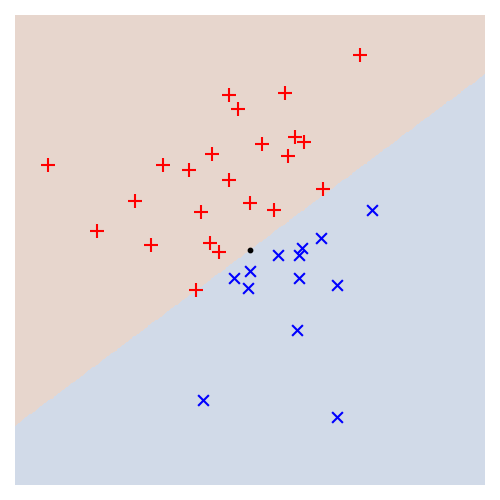
\includegraphics[height=1.9cm]{db-linr-a}
                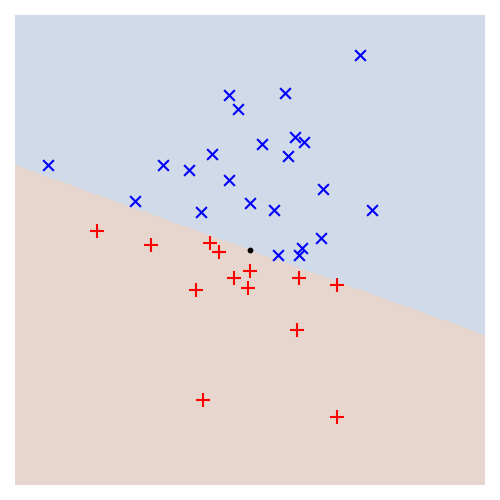
\includegraphics[height=1.9cm]{db-linr-b}
                \caption{\emph{
                    Two $f$s in $\Hh_{\text{lin}}$.
                    A line through the origin divides the plane ($\Xx=\RR^2$)
                    into red (Cow) and blue (Dog) parts.  We also show how each
                    $f$ classifies some random points.
                }}
                \label{fig:linr}
            \end{marginfigure}}%
            Here, $\text{sign}$ sends negative numbers to Dog and positive
            numbers to Cow.  Let's not worry about the boundary case of $0$
            except to note that images on which $\theta$ is $0$ together
            form a \textbf{decision boundary} between the Cows and the Dogs.

            The jaggedness of $\Hh$ is at most $d$, because any $d+1$ points
            $x_0, x_1,\cdots x_d \in \RR^d$ must participate in some linear
            relation:
            $$
                x_s = 
                \sum_{i\in I} c_i x_i
                -
                \sum_{j\in J} c_j x_j
            $$
            {\def\par{\let\par\endgraf}\begin{marginfigure}
                \centering
                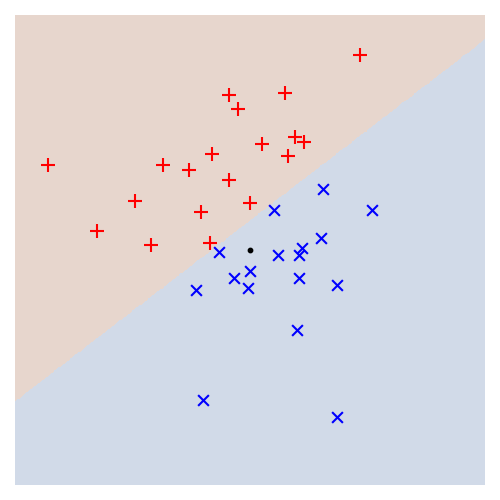
\includegraphics[height=1.9cm]{db-bias-a}
                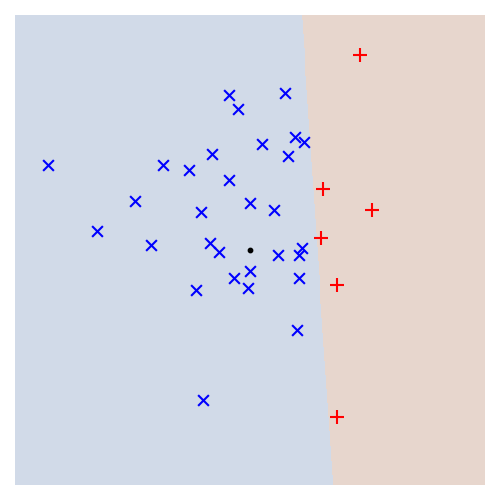
\includegraphics[height=1.9cm]{db-bias-b}
                \caption{\emph{
                    Decision boundaries with bias may avoid the origin.
                }}
                \label{fig:bias}
            \end{marginfigure}}
            for some $\{s\},I,J$ mutually disjoint and each $c$ positive.
            Thus, if we assign to each $x_i$ a positive label (Cow) and to each
            $x_j$ a negative label (Dog), then $x_s$ must have a positive label
            (Cow).  Therefore, not all $2^d$ possibilities occur.  As long
            as $\sqrt{\log(N)\cdot d/N}$ is small, learning with
            $\Hh_{\text{lin}}$ will generalize.

            \begin{marginfigure}
                \centering
                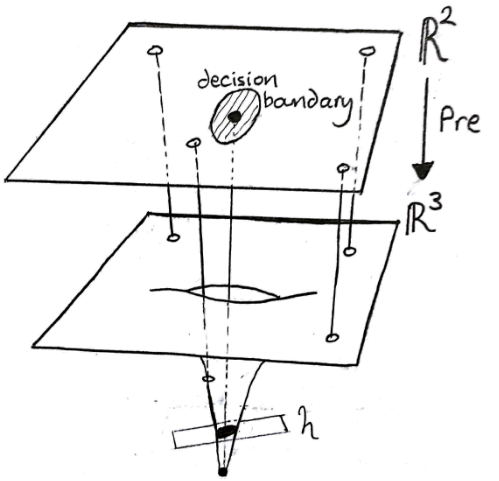
\includegraphics[height=3.0cm]{transform-two-three}
                \caption{\emph{
                    Linear planes (bottom) in the transformed $\Xx$ induce
                    non-linear boundaries (top) in the old $\Xx$.
                }}
            \end{marginfigure}
            By the way, what if
            %lines through the origin don't make
            %sense for our classification problem?  For example, what if
            we want
            to model decision boundaries that don't pierce the origin?
            Well, one trick is to \textbf{pre-process} the data so that linear
            classification of the transformed data corresponds to richer
            classification of the old data.  If we map
            $$
                \text{old features} = (a,b)
                \mapsto
                \text{new features} = (1, a, b)
            $$
            then boundaries may avoid the origin (Figure
            \ref{fig:bias}).  This is called ``adding a \textbf{bias} term''.
            Instead of classifying points in $\Xx=\RR^2$, we now classify
            points in $\Xx=\RR^3$, meaning that our jaggedness is $3$ instead
            of $2$ and generalization may be a bit worse.
            %

            The same trick gives us curvy boundaries.
            For example, we might use polynomials
            $$
                \text{old features} = (a, b)
                \mapsto
                \text{new features} = (1, a, b, a^2, ab, b^2, a^3, a^2b, ab^2, b^3)
            $$
            {\def\par{\let\par\endgraf}\begin{marginfigure}
                \centering
                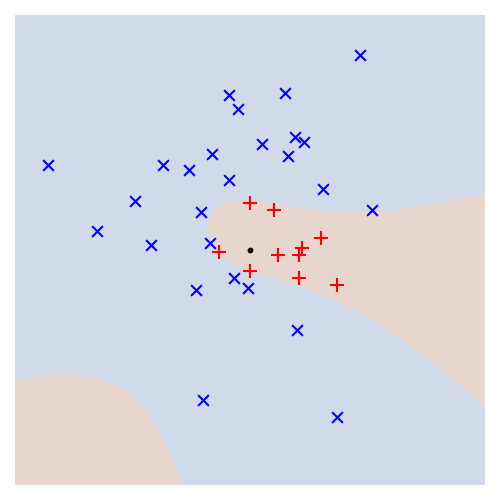
\includegraphics[height=1.9cm]{db-cubc-a}
                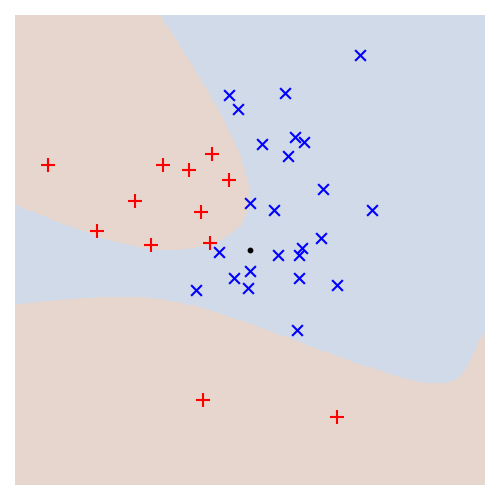
\includegraphics[height=1.9cm]{db-cubc-b}
                \caption{\emph{
                    Polynomial features allow decision boundaries to exhibit
                    peninsulas, channels, and islands.
                }}
                \label{fig:cubc}
            \end{marginfigure}}%
            to get decision boundaries as in Figure \ref{fig:cubc}.
            Instead of classifying points in $\Xx=\RR^2$, we
            now classify points in $\Xx=\RR^{10}$, meaning that our jaggedness
            is $10$ instead of $2$ and generalization may be substantially
            worse.



            \newpage
        \section{Optimization}
            How do we select $f\in \Hh_{\text{lin}}$ based on the data
            $\Ss$?  Since the jaggedness $d$ is finite, it makes sense to
            seek an $f$ with low training error:
            $$
                N \cdot \Ein(\theta) =
                    \sum_{(x,\text{Cow})\in \Ss}
                    \begin{cases} 
                        1       &       \text{if}~\theta(x) < 0 \\
                        0       &       \text{otherwise}
                    \end{cases}
                    + 
                    \sum_{(x,\text{Dog})\in \Ss}
                    \begin{cases} 
                        1       &       \text{if}~\theta(x) > 0 \\
                        0       &       \text{otherwise}
                    \end{cases}
            $$
            Now, a general strategy to find a good $f$ is to start with some
            $f$ and to keep replacing it with better $f$'s.
            %
            The problem is that each point is either misclassified or not,
            so we don't have a very gradual notion of improvement.
            %The problem is that $\Ein(f)$ takes discrete values $0/N$, $1/N$,
            %$\cdots$, $N/N$, so it is hard to tell in which direction we should
            %nudge $f$ to improve it.

            Imagine the true label is Cow, so we want
            $\theta(x)>0$, but currently
            $\theta(x) = -0.20$.  Intuitively, $\theta(x)=-0.15$ is an
            improvement, even though it is still a misclassification.
            Likewise, $\theta(x)=+0.05$ is precariously close to
            negative.
            Therefore, let's take small steps to improve a notion
            of \textbf{badness} according to which $-0.20$ is
            worse than $-0.15$ is worse than $0.05$ is worse than $1.00$.  At
            some point, we consider $\theta(x)$ safe instead of precarious;
            let's say $1.00$ is no worse than $1.05$.
            %
            We write this as a formula:\footnote{
                There are lots of ways to turn the qualitative pattern we 
                discussed into a formula.  What we present is called
                \textbf{hinge loss}.  Our favorite way, \textbf{logistic
                loss}, has a beautiful probabilistic interpretation,
                but we won't have time to talk about it.
            }
            \begin{align*}
                \text{badness}(\theta) = 
            {\small
                    \sum_{(x,\text{Cow})\in \Ss}
                    \begin{cases} 
                        1-\theta(x)    &   \text{if}~\theta(x) < +1 \\
                        0              &   \text{otherwise}
                    \end{cases}
                    +
                    \sum_{(x,\text{Dog})\in \Ss}
                    \begin{cases} 
                        1+\theta(x)    &   \text{if}~\theta(x) > -1\\
                        0              &   \text{otherwise}
                    \end{cases}
            }
            \end{align*}
            Each term of $\text{badness}$ exceeds the
            corresponding term of $N\cdot \Ein$.  Minimizing badness thus
            makes sense as an approximate way to minimize $\Ein$.

            %The upshot is that we can make incremental improvements with small
            %steps.
            What's the difference between
            $\text{badness}(\theta)$ and 
            $\text{badness}(\theta+\epsilon)$, where $\epsilon$ is a ``small''
            linear function?
            %
            Each of the non-zero terms changes by
            $\epsilon(x)$ when we change $\theta$ into $\theta+\epsilon$.  
            So the net decrease in badness is:\footnote{
                Well, actually this isn't exactly right, since whether we use
                the ``ifs'' of the ``otherwises'' might change between $\theta$
                and $\theta + \epsilon$.  We imagine that $\epsilon$ is so
                small that this is negligible.  That's what we mean by ``small'',
                and that's why we write $\approx$ instead of $=$.
            }
            \begin{align*}
                \text{improvement}
                &\approx
                    \sum_{(x,\text{Cow})\in \Ss}
                    \begin{cases} 
                        \epsilon(x)      &       \text{if}~\theta(x) < +1 \\
                        0                &       \text{otherwise}
                    \end{cases}
                    +\sum_{(x,\text{Dog})\in \Ss}
                    \begin{cases} 
                        -\epsilon(x)     &       \text{if}~\theta(x) > -1\\
                        0                &       \text{otherwise}
                    \end{cases}
                    \\
                &=
                    \epsilon\left(
                        +
                        \sum_{\substack{(x,\text{Cow})\in \Ss \\ \text{and}~\theta(x)<+1}} x
                        -
                        \sum_{\substack{(x,\text{Dog})\in \Ss \\ \text{and}~\theta(x)>-1}} x
                    \right)
                = \epsilon(x_{\text{squeaky}})
            \end{align*}
            Above, we used $\epsilon$'s linearity then renamed its input
            $x_{\text{squeaky}}$ to save ink.\footnote{
                After all, each term in $x_{\text{squeaky}}$ is
                (or is precariously close to being) 
                misclassified.
                And you know what they say: \emph{the squeaky wheel gets the grease}.
            }

            So for every possible value of the vector $x_{\text{squeaky}}$,
            want to find some $\epsilon = \eta(x_{\text{squeaky}})$ such that
            the improvement $\approx \epsilon(x_{\text{squeaky}}) =
            \eta(x_{\text{squeaky}})(x_{\text{squeaky}})$ is positive.
            A large
            class of useful $\eta$s are the \textbf{inner products}.
            Different inner products will select different $f$s from among the
            tied best $f$s.

            %            Overall, our algorithm looks like: 
            %            \begin{lstlisting}[mathescape, basicstyle=\ttfamily]
            %    Initialize $\theta$ to $0$
            %    Repeat many times:
            %        Use the current $\theta$ to classify the training data
            %        Add up the misclassified points to get $x_{\text{squeaky}}$
            %        Update $\theta$ to $\theta + \eta(x_{\text{squeaky}})$
            %            \end{lstlisting}


            %How shall we choose a small linear function
            %$\epsilon$ that makes an improvement?  There are lots of choices,
            %and each leads to a different algorithm.  If we write out input
            %data in coordinates, like $x = (x_a,x_b,x_c, \cdots)$, then one way is
            %to define:
            %$$
            %    \epsilon(y) = 0.03 \cdot x_a y_a + 0.02 \cdot x_b y_b +
            %                    0.01 \cdot x_a y_b + 0.01 \cdot x_c y_c + \cdots
            %$$
            %We chose small coefficients to ensure that $\epsilon$ is ``small'',
            %and as long as the coefficients of the cross terms like $0.01 \cdot x_a
            %y_b$ are close to $0$, this formula will guarantee that the
            %improvement  $\epsilon(x_{\text{squeaky}})$ is positive.

    \newpage
    \chapter{Example: Classifying Clothing}
        \section{Featurization}
            \begin{figure}
                \centering
                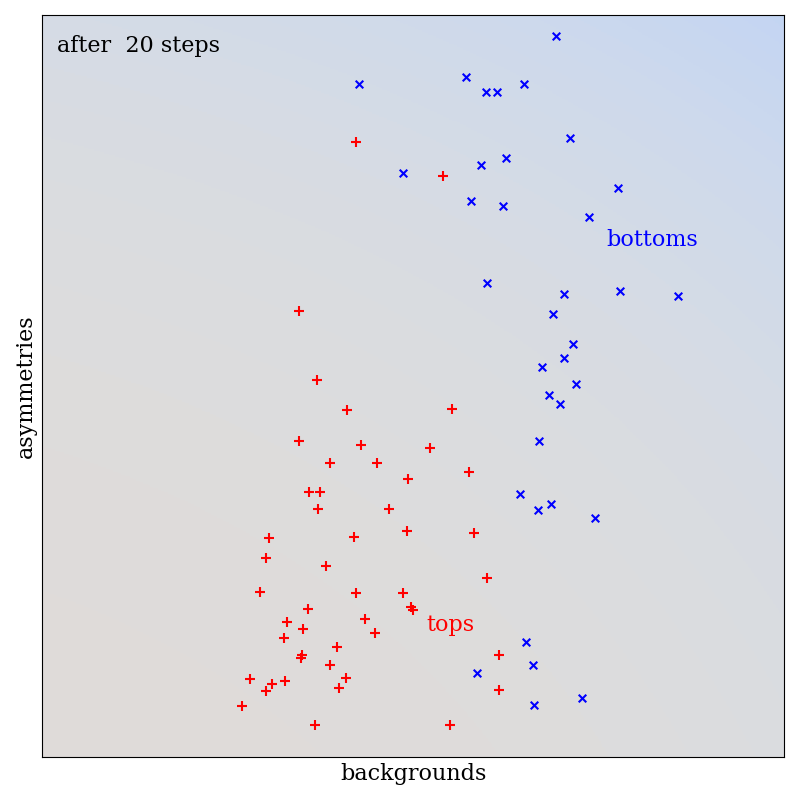
\includegraphics[height=3.9cm]{yo-00-sm}
                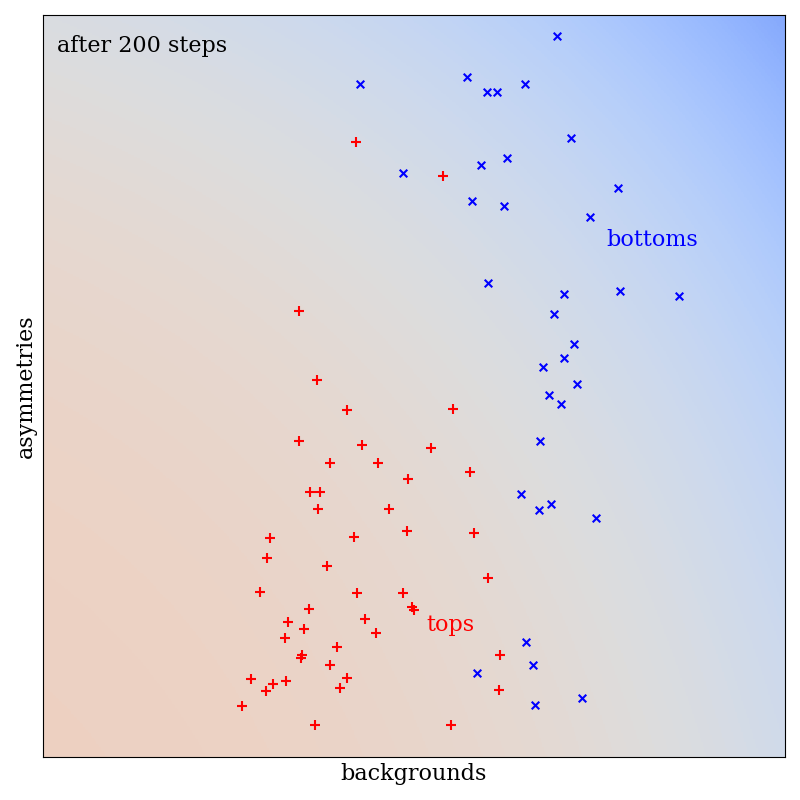
\includegraphics[height=3.9cm]{yo-03-sm}
                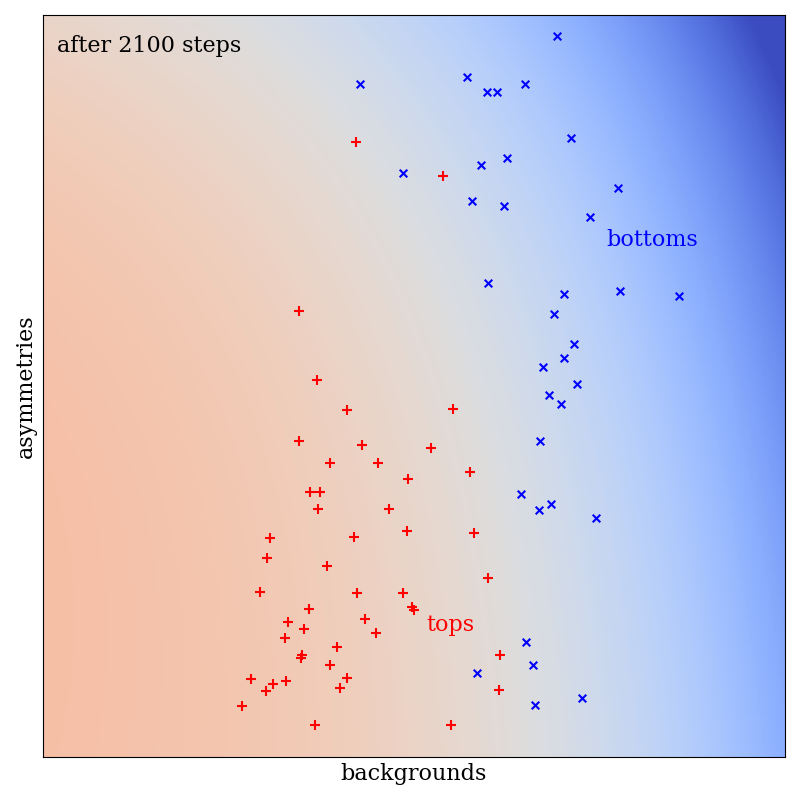
\includegraphics[height=3.9cm]{yo-13-sm}\\
                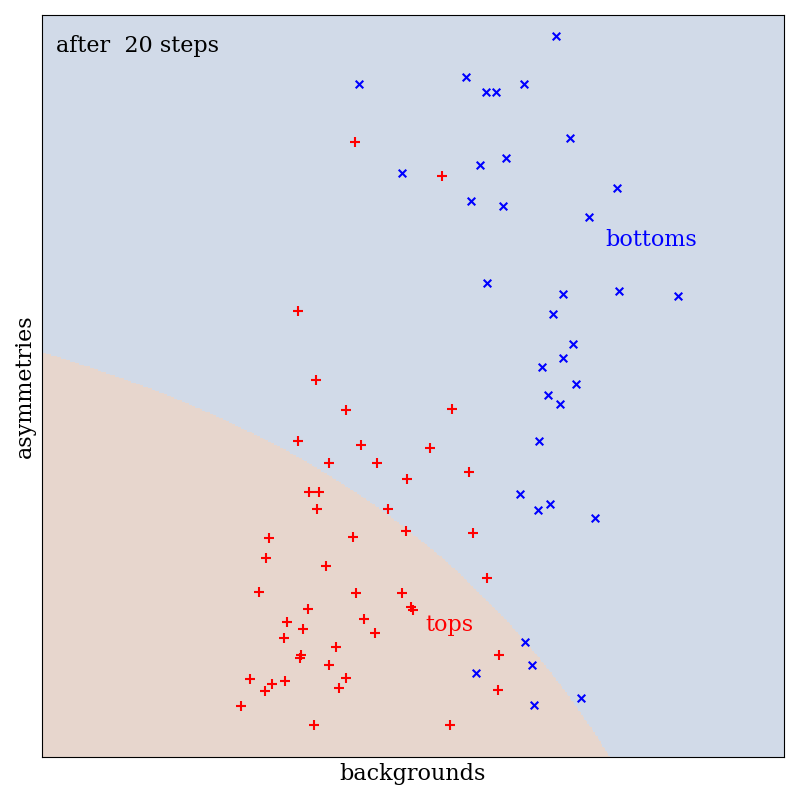
\includegraphics[height=3.9cm]{yo-00-bd}
                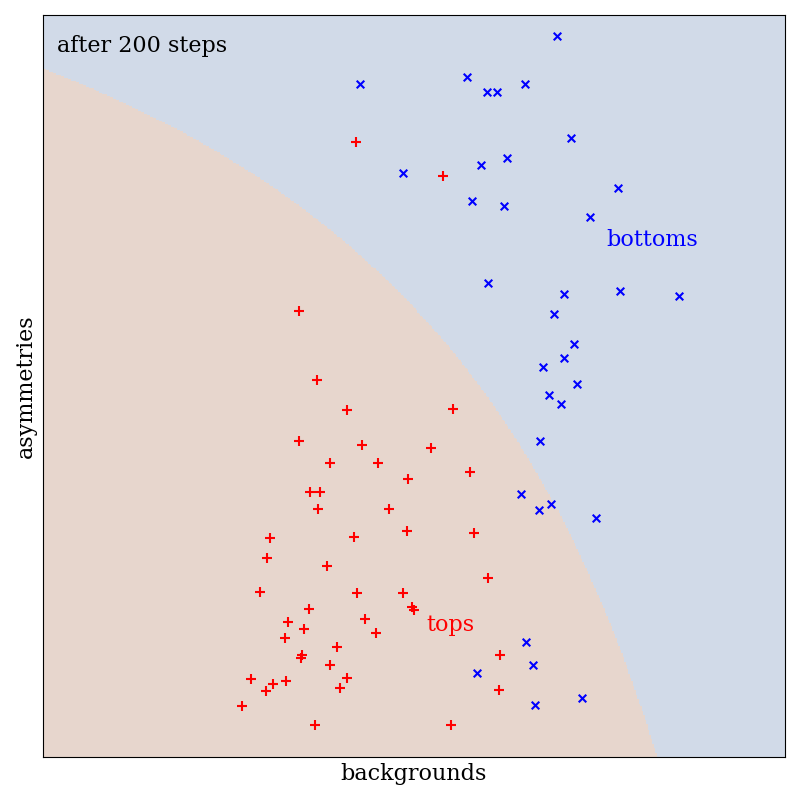
\includegraphics[height=3.9cm]{yo-03-bd}
                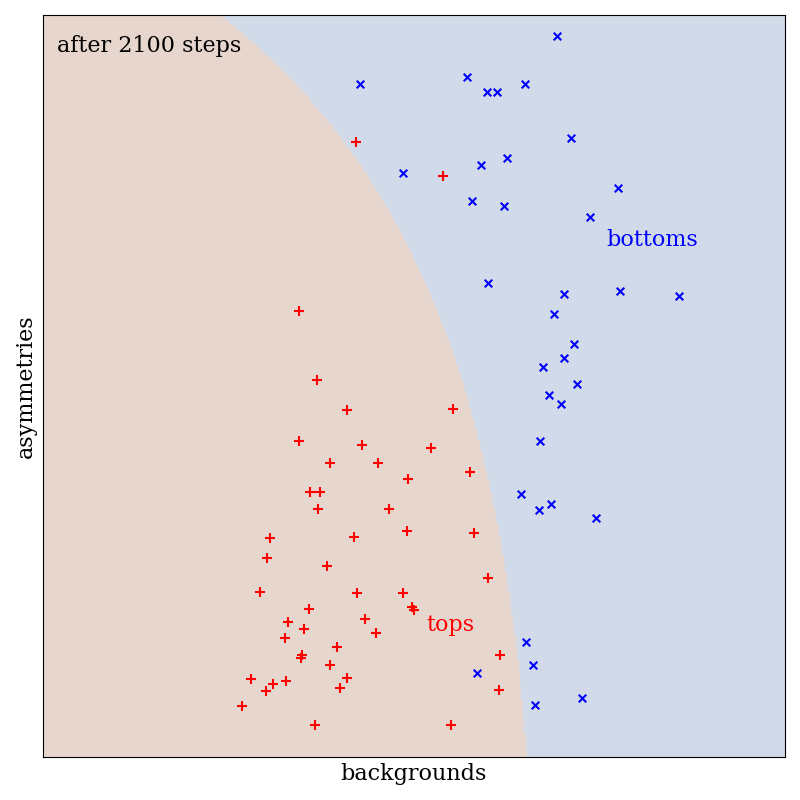
\includegraphics[height=3.9cm]{yo-13-bd}
                \caption{\emph{
                    Polynomial features allow decision boundaries to exhibit
                    peninsulas, channels, and islands.
                }}
            \end{figure}

        \section{Learning Curves}


    %\newpage
    %\chapter{Regularization}
    %    %\section{Rademacher complexity}
    %    %\section{Margin bounds}

    %\chapter{Structure in $\Dd$}
    %    \section{Rademacher Complexity}
    %    \section{Margin Bounds}

    %\chapter{Structure in $\Ll$}
    %    \section{Privacy and Generalization}
    %    \section{The Akaike Information Criterion and its Cousins}

    %\chapter{Frame Conditions and Independence}
    %    \section{Simplicity and Subjectivity}
    %    \section{Independence in Practice?}



    %\newpage
    %\chapter*{Helping Handout: Binomial Coefficients ${n \choose k}$}
    %    How many ways can we select $k$ people out of $n$ people?
    %    For example,
    %    there is just $1$ way to choose a pair ($k=2$) from among $n=2$ people.
    %    There are $3$ pairs among $n=3$ people.
    %    And there are $6$ pairs among $n=4$ people.
    %    We write the answer to this question as ${n\choose k}$; so
    %    ${4\choose 2} = 6$. 
    %    
    %    While ${n\choose k}$ counts size-$k$ subsets, so that picking Alice 
    %    and Bob is the same as picking Bob and Alice, we might want to count
    %    ordered subsets.
    %    How about if we want to order $k=4$ people out of $n=10$ people?
    %    Well, there are $10$ ways to select the first person,
    %                     $9$ ways to select the second person,
    %                     $8$ ways to select the third person, and
    %                     $7$ ways to select the fourth person.
    %    So the answer is $10\cdot 9\cdot 8\cdot 7$.
    %    But each size-$k$ unordered subset corresponds to
    %    $4\cdot 3\cdot 2\cdot 1$ ordered subsets.  So we conclude that
    %    $$
    %        {10\choose 4} = \frac{10\cdot 9\cdot 8\cdot 7}{4\cdot 3\cdot 2\cdot 1} 
    %    $$

    %    Notice that ${n \choose 0} = 1$, since there is always exactly one way
    %    to choose none of the $n$ people.
    %    %
    %    Also, when $n$ is positive, ${n\choose k} = {n-1\choose k-1} +
    %    {n\choose k-1}$, since to choose $k$ folks from among a group of $n-1$
    %    students and $1$ teacher, we can \textbf{either} choose $k$ students
    %    and leave out the teacher \textbf{or} choose $k-1$ students and also
    %    the teacher.
    %    %
    %    Another neat fact is that
    %    $
    %        {n\choose 0} + {n\choose 1} + {n\choose 2} + \cdots + {n\choose k}
    %        = 2^n
    %    $
    %    as long as $n\leq k$.  This is because that sum
    %    counts the number of ways to choose some subset of size at
    %    most $k$ from among $n$ people.  

    %\chapter*{Helping Handout: Asymptotics}

    %\newpage
    %\chapter*{Helping Handout: Probability}
    %    How can we model the notion of \textbf{chance} using math?
    %    For example, we might have a set $\Xx=[0\,\text{cm}, 50\,\text{cm}]$ of
    %    possible daily rainfall levels.  Intuitively, there is zero chance that
    %    any particular positive rainfall like $6.28318\cdots\,\text{cm}$ will
    %    occur today.  But we'd say there is some chance that the rainfall will
    %    fall within, say, $[6.2\,\text{cm}, 6.3\,\text{cm}]$.
    %    %
    %    Thus, in order to treat $\Xx$ probabilistically, we want to assign to
    %    each interval $I \subseteq \Xx$ a nonnegative number $\PP(I)$ that
    %    tells us the chance that rainfall will fall within $I$.  In order for
    %    this bunch of numbers to make sense, we demand $\PP(\Xx)=1$ and that,
    %    whenever a bunch of intervals $I_0, I_1, \cdots$ partition a bigger
    %    interval $J$, then $\PP(I_0) + \PP(I_1) + \cdots = \PP(J)$.
    %    By the way, it is convenient to think of $\PP$ as defined on unions of
    %    disjoint intervals instead of intervals.

    %    In general, a \textbf{probability distribution} on a set $\Xx$ is a
    %    bunch of ``generalized unions-of-intervals'' of ``events'' that are subsets of $\Xx$,
    %    each labeled by a nonnegative number, that
    %    follows the above demands.  Precisely, the data is: a collection $\Ii
    %    \subseteq 2^\Xx$ of subsets of $\Xx$ and a function $\PP:\Ii\to [0,
    %    1]$, such that the following are well-defined and true whenever $I,
    %    I_0, I_1, \cdots \in \Ii$.
    %    $$ 
    %        \PP(\Xx - I) + \PP(I) = \PP(\Xx) = 1 
    %    $$
    %    and
    %    $$
    %        \PP(I_0) + \PP(I_1) + \cdots = \PP(I_0 \cup I_1 \cup \cdots)
    %        ~~~~~
    %        \text{when the $I$'s are disjoint}
    %    $$

    %    One technique to understand complicated events is to break them up
    %    into simpler events.  For example, it is intuitive that the chance that
    %    a coin lands heads while a die lands sixes is related to the separate
    %    chances that a coin lands heads and that a die lands sixes.  In particular,
    %    we expect heads to occur $1/2$ of the time and sixes to occur $1/6$ of
    %    the time, and thus both together to occur $(1/2) \cdot (1/6) = 1/12$ of
    %    the time.  When simple events compose this way, we call them
    %    \textbf{independent}:
    %    $$
    %        \PP(I_0 \cap I_1 \cap \cdots) = \PP(I_0) \cdot \PP(I_1) \cdot \cdots
    %        ~~~~~
    %        \text{when $I_0, I_1, \cdots$ are independent} 
    %    $$
    %    Events aren't always independent though.  In general, we may define
    %    symbols $\PP(I | J)$ for the \textbf{conditional probability} that $I$
    %    happens assuming that $J$ happens:
    %    $$
    %        \PP(I \cap J) = \PP(I | J)\cdot \PP(J)
    %    $$
    %    There is exactly one choice for $\PP(I|J)$ when $\PP(J)\neq 0$.
    %    we may choose $\PP(I|J)=\PP(I)$ exactly when $I, J$ are independent.
    %    %
    %    Conditional probabilities formalize ``what if'' questions:
    %    For example, what is the chance that of $\geq 2\,\text{cm}$ of rain
    %    given $\geq 1\,\text{cm}$ of rain?  

    %    \section*{Monty Hall}
    %        Here's a practice example.  Imagine three boxes, exactly
    %        one of which contains a prize.  We don't know which.
    %        We play a game that has three steps: First, we pick a box.  Next, a
    %        gameshow host removes one of the empty boxes that isn't the box we
    %        picked.  Finally, we are allowed to pick one of the two remaining
    %        boxes; it will either be our original box, or a different box.  If
    %        this final pick contains the prize, then we win.

    %        Here are three strategies we might use:
    %        \textbf{stay} --- we pick the original box; or
    %        \textbf{swap} --- we pick the different box; or
    %        \textbf{flip} --- based on a flip of a fair coin, we pick the original or different box.

    %        The \textbf{stay} strategy has a $1/3$ chance of winning, since 
    %        playing the game with this strategy leads us to choose the prize
    %        box as much as one empty box as much as the other empty box.

    %        The \textbf{flip} strategy has a $1/2$ chance of winning, since 
    %        playing the game with this strategy leads us to choose the prize
    %        box as much as the empty remaining box.

    %        And $\PP_{\textbf{flip}}(\text{win})$ is the average of 
    %        $\PP_{\textbf{stay}}(\text{win})$ and
    %        $\PP_{\textbf{swap}}(\text{win})$.
    %        Therefore, the \textbf{swap} strategy has a $2/3$ chance of
    %        winning.  It is by far the best.

    %\chapter*{Helping Handout: Vectors and Covectors}
    
%        \section{Cross entropy}
%
%            Suppose we know a selfish expert who knows the true probability $p$   
%            of a hurricane happening this month.  We want to incentivize the
%            expert to tell us $p$ beforehand.  The expert tells us
%            some number $\hat p$ when we ask them, and we want to penalize them
%            at the end of the month so that it is in their best interests to
%            say the true $p$.
%
%            Ideally, we would reward the expert according to whether $\hat p$
%            matches the true $p$.  The problem is, even at the end of the
%            month, we won't know the true $p$!  All we know is whether or not a
%            hurricane happened --- this is related to $p$ but not the same.
%            So we want some reward functions
%            $l_{\text{wet}}(\hat p)$ and
%            $l_{\text{dry}}(\hat p)$ 
%            to be handed out depending on whether a hurricane happens.
%            Hmm... is this even possible?
%
%            Yes!  The marvelous miracle is that the following reward functions
%            work!
%            $$
%                l_{\text{wet}}(\hat p,\hat q) = \log(\hat p)~\text{dollars}
%                ~~~~~
%                ~~~~~
%                ~~~~~
%                l_{\text{dry}}(\hat p,\hat q) = \log(\hat q)~\text{dollars}
%            $$
%
%            Here's one way to see this.  The reward after $N$ independent
%            trials over will be around $Np \log(\hat p) + Nq \log(\hat q)$,
%            which is:
%            $$
%                \log( \hat p^{Np} \cdot \hat q^{Nq} )
%            $$
%            The quantity inside the $\log$ is just the probability that, if
%            we flip a $\hat p$-biased coin $N$ times, then we see $Np$ heads
%            in a row and then $Nq$ tails in a row.  It is intuitive that the
%            value of $\hat p$ that makes this outcome most likely is
%            $\hat p = p$.
%
%            In fact, if we don't count silly variations,\footnote{
%                namely, scaling (using cents instead of dollars) and shifting
%                (gifting an extra amount that doesn't depend
%                on $\hat p, \hat q$)
%            } the above penalty system is the unique one that works!

%            What we do instead is to consider candidates that estimate the
%            probability of being a Cow rather than estimate an absolute label:
%            $$
%                \Hh = \{
%                    x \mapsto (\exp(\theta(x))\text{-to-}1~\text{odds of Cow})
%                    ~\text{where}~
%                    \theta : \RR^d \to \RR
%                    ~\text{is linear}
%                \}
%            $$
%            From the point of view of $f\in \Hh$, the likelihood of a datapoint
%            $x$ being labeled Dog (or Cow) is
%            $
%                1/(\exp(\theta(x)) + 1)
%            $ (or one minus that).  And the likelihood of the training set
%            overall is a big product of likelihoods.  It is reasonable to shift
%            our goals to maximize this likelihood rather than $\Ein$.  Since
%            likelihood varies smoothly as $\theta$ varies, we may start with an
%            arbitrary $\theta\in \Hh$ and then take small steps, each time
%            finding a slightly different $\theta$ from whose perspective the
%            fixed training data is more likely.
%
%            Let's see how this works in more detail.  If we have
%            $3$ datapoints $(x,Cow), (y,Dog), (z,Dog)$, then the likelihood is
%            $$
%                L = 
%                \frac{\exp(\theta(x))}{\exp(\theta(x)) + 1}
%                \cdot
%                \frac{1}{\exp(\theta(y)) + 1}
%                \cdot
%                \frac{1}{\exp(\theta(y)) + 1}
%            $$
%            Now if we change $\theta$ to $\theta+\epsilon$ for some small
%            linear function $\epsilon$, then $\exp((\theta+\epsilon))(x)$  




\end{document}


